\documentclass[norsk, 12pt]{beamer}
% Add handout to documentclass options if wanted

\usepackage[latin1]{inputenc}
\usepackage[T1]{fontenc}
\usepackage{babel,textcomp}

\setlength{\arrayrulewidth}{1.6pt}
\renewcommand{\arraystretch}{1.2}
\newlength{\Tcalc}

\usepackage[T1]{fontenc}
\usepackage{graphicx}
\usepackage{amsmath}
\usepackage{amssymb}
\usepackage{amsbsy}
\usepackage{amsfonts}
\usepackage{color}
\usepackage{xcolor}
\usepackage{epstopdf}
\usepackage{fancyvrb}
\usepackage{parskip}
\usepackage{url}
\usepackage{listings}

\definecolor{javared}{rgb}{0.6,0,0} % for strings
\definecolor{javagreen}{rgb}{0.25,0.5,0.35} % comments
\definecolor{javapurple}{rgb}{0.5,0,0.35} % keywords
\definecolor{javadocblue}{rgb}{0.25,0.35,0.75} % javadoc

\lstset{language=Matlab,
basicstyle=\ttfamily
keywordstyle=\color{javapurple},%\bfseries,
stringstyle=\color{javared},
commentstyle=\color{javagreen},
morecomment=[s][\color{javadocblue}]{/**}{*/},
morekeywords={super, with},
% numbers=left,
% numberstyle=\tiny\color{black},
stepnumber=2,
numbersep=10pt,
tabsize=2,
showspaces=false,
% captionpos=b,
showstringspaces=false,
frame=  false,
breaklines=true}

\setbeamertemplate{frametitle}
{\begin{centering}\smallskip
\insertframetitle\par
\smallskip\end{centering}}
\setbeamertemplate{itemize item}{$\bullet$}
\setbeamertemplate{navigation symbols}{}
\setbeamertemplate{footline}[text line]{%
\hfill\strut{%
\scriptsize\sf\color{black!60}%
\quad\insertframenumber
   }%
    \hfill
}

% Define some colors:
\definecolor{DarkFern}{HTML}{407428}
\definecolor{DarkCharcoal}{HTML}{4D4944}
\colorlet{Fern}{DarkFern!85!white}
\colorlet{Charcoal}{DarkCharcoal!85!white}
\colorlet{LightCharcoal}{Charcoal!50!white}
\colorlet{AlertColor}{orange!80!black}
\colorlet{DarkRed}{red!70!black}
\colorlet{LightBlue}{blue!70!white}
\colorlet{DarkBlue}{blue!70!black}
\colorlet{DarkGreen}{green!70!black}

% Use the colors:
\setbeamercolor{title}{fg=Fern}
\setbeamercolor{frametitle}{fg=Fern}
\setbeamercolor{normal text}{fg=Charcoal}
\setbeamercolor{block title}{fg=black,bg=Fern!25!white}
\setbeamercolor{block body}{fg=black,bg=Fern!25!white}
\setbeamercolor{alerted text}{fg=AlertColor}
\setbeamercolor{itemize item}{fg=Charcoal}

\newcommand{\frn}[1]{\textcolor{Fern}{#1}}
\newcommand{\alrt}{\color{AlertColor}}
\newcommand{\bt}[1]{\textbf{#1}}
\newcommand{\kommando}[1]{\textcolor{AlertColor}{\texttt{\textbackslash #1}}}
\newcommand{\ds}{\displaystyle}

\title{Studies of near-gaussian beams}
\author{Jonas van den Brink}
\institute{}
\date{1. desember 2014}

\setbeamertemplate{frametitle}{\vspace{0.5cm} \insertframetitle} 

\begin{document}
\pagestyle{empty}

\section{Introduksjon}

\begin{frame}[fragile]
\begin{center}	
{\Huge \color{DarkFern} Studies of near-gaussian beams}
\begin{center}
\vspace{0.1cm}
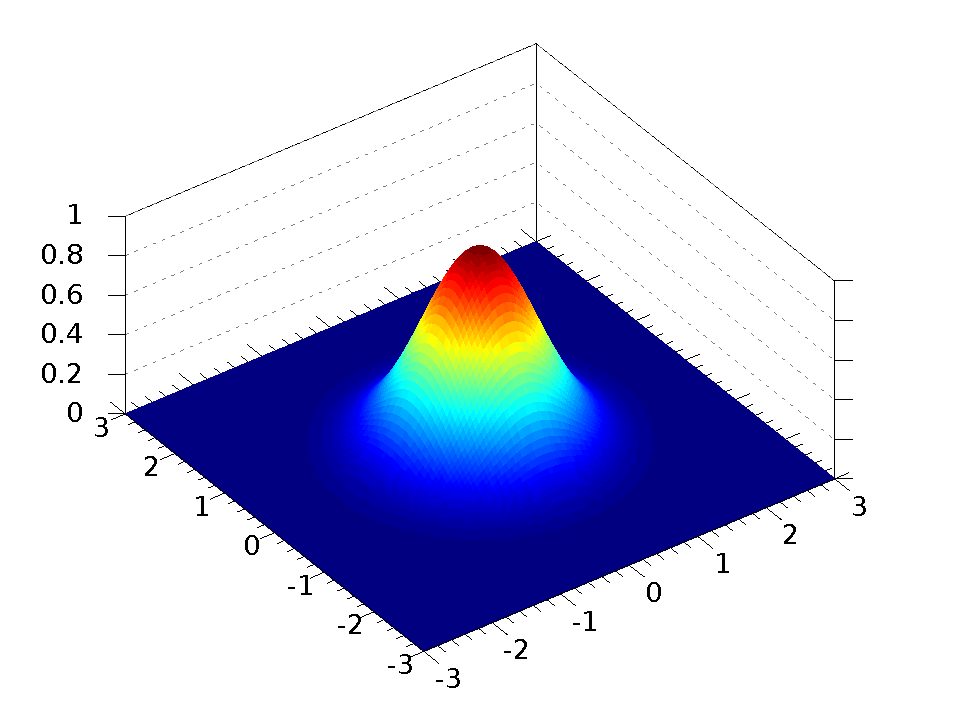
\includegraphics[width=0.7\textwidth]{Gaussian_2d.pdf}
\vspace{0.1cm}
\end{center}
{\centering \color{Charcoal} Jonas van den Brink}
\end{center}
\end{frame}


\begin{frame}[fragile]
{\large \color{DarkFern} Ingen laserstr�le har konstant bredde}
\begin{center}
\vspace{0.2cm}
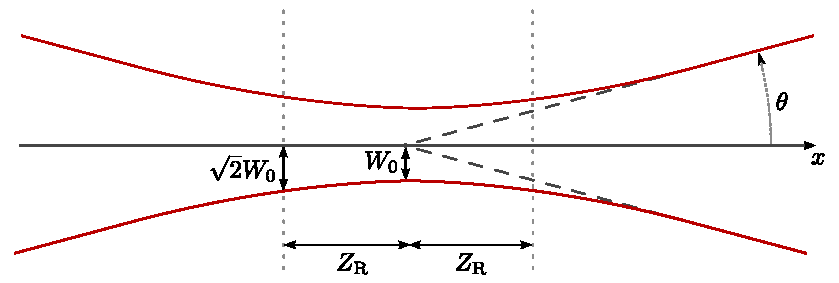
\includegraphics[width=\textwidth]{beam.pdf}
\vspace{0.2cm}
\visible<2->{For en gaussisk beam har vi
 $\theta = \dfrac{\lambda}{\pi w_0}.$}

\vspace{0.2cm}
\visible<3->{Definerer str�lekvalitet $$\mbox{BPP} =\theta \cdot w_0, \qquad M^2 = \frac{\mbox{BPP}}{\mbox{BPP}_{\mbox{G}}}.$$}
\end{center}
\end{frame}


\begin{frame}[fragile]
{\large \color{DarkFern} Linser endrer krumningsradien}
\begin{center}
\vspace{0.2cm}
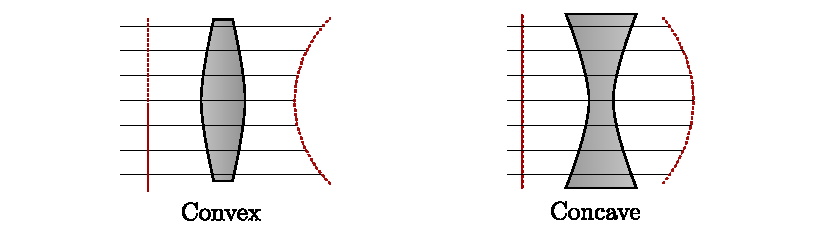
\includegraphics[width=\textwidth]{lenses.pdf}
\end{center}
\end{frame}

\begin{frame}[fragile]
{\large \color{DarkFern} Vi kan lage en beam expander fra to bikonvekse linser}
\begin{center}
\vspace{0.2cm}
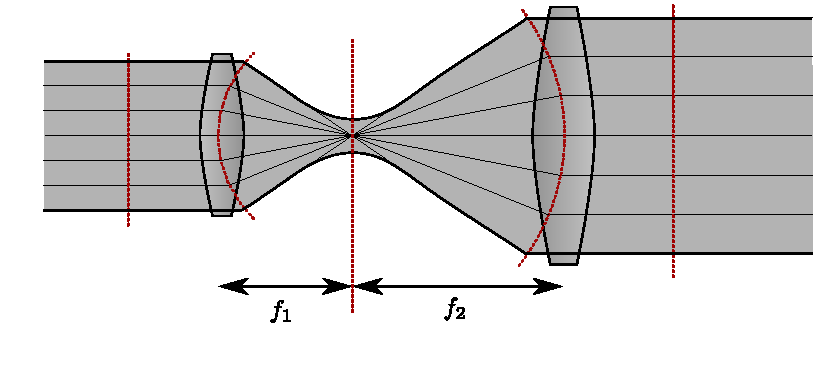
\includegraphics[width=\textwidth]{beam_expander.pdf}
\end{center}
\end{frame}

\begin{frame}[fragile]
\begin{center}
\vspace{0.2cm}
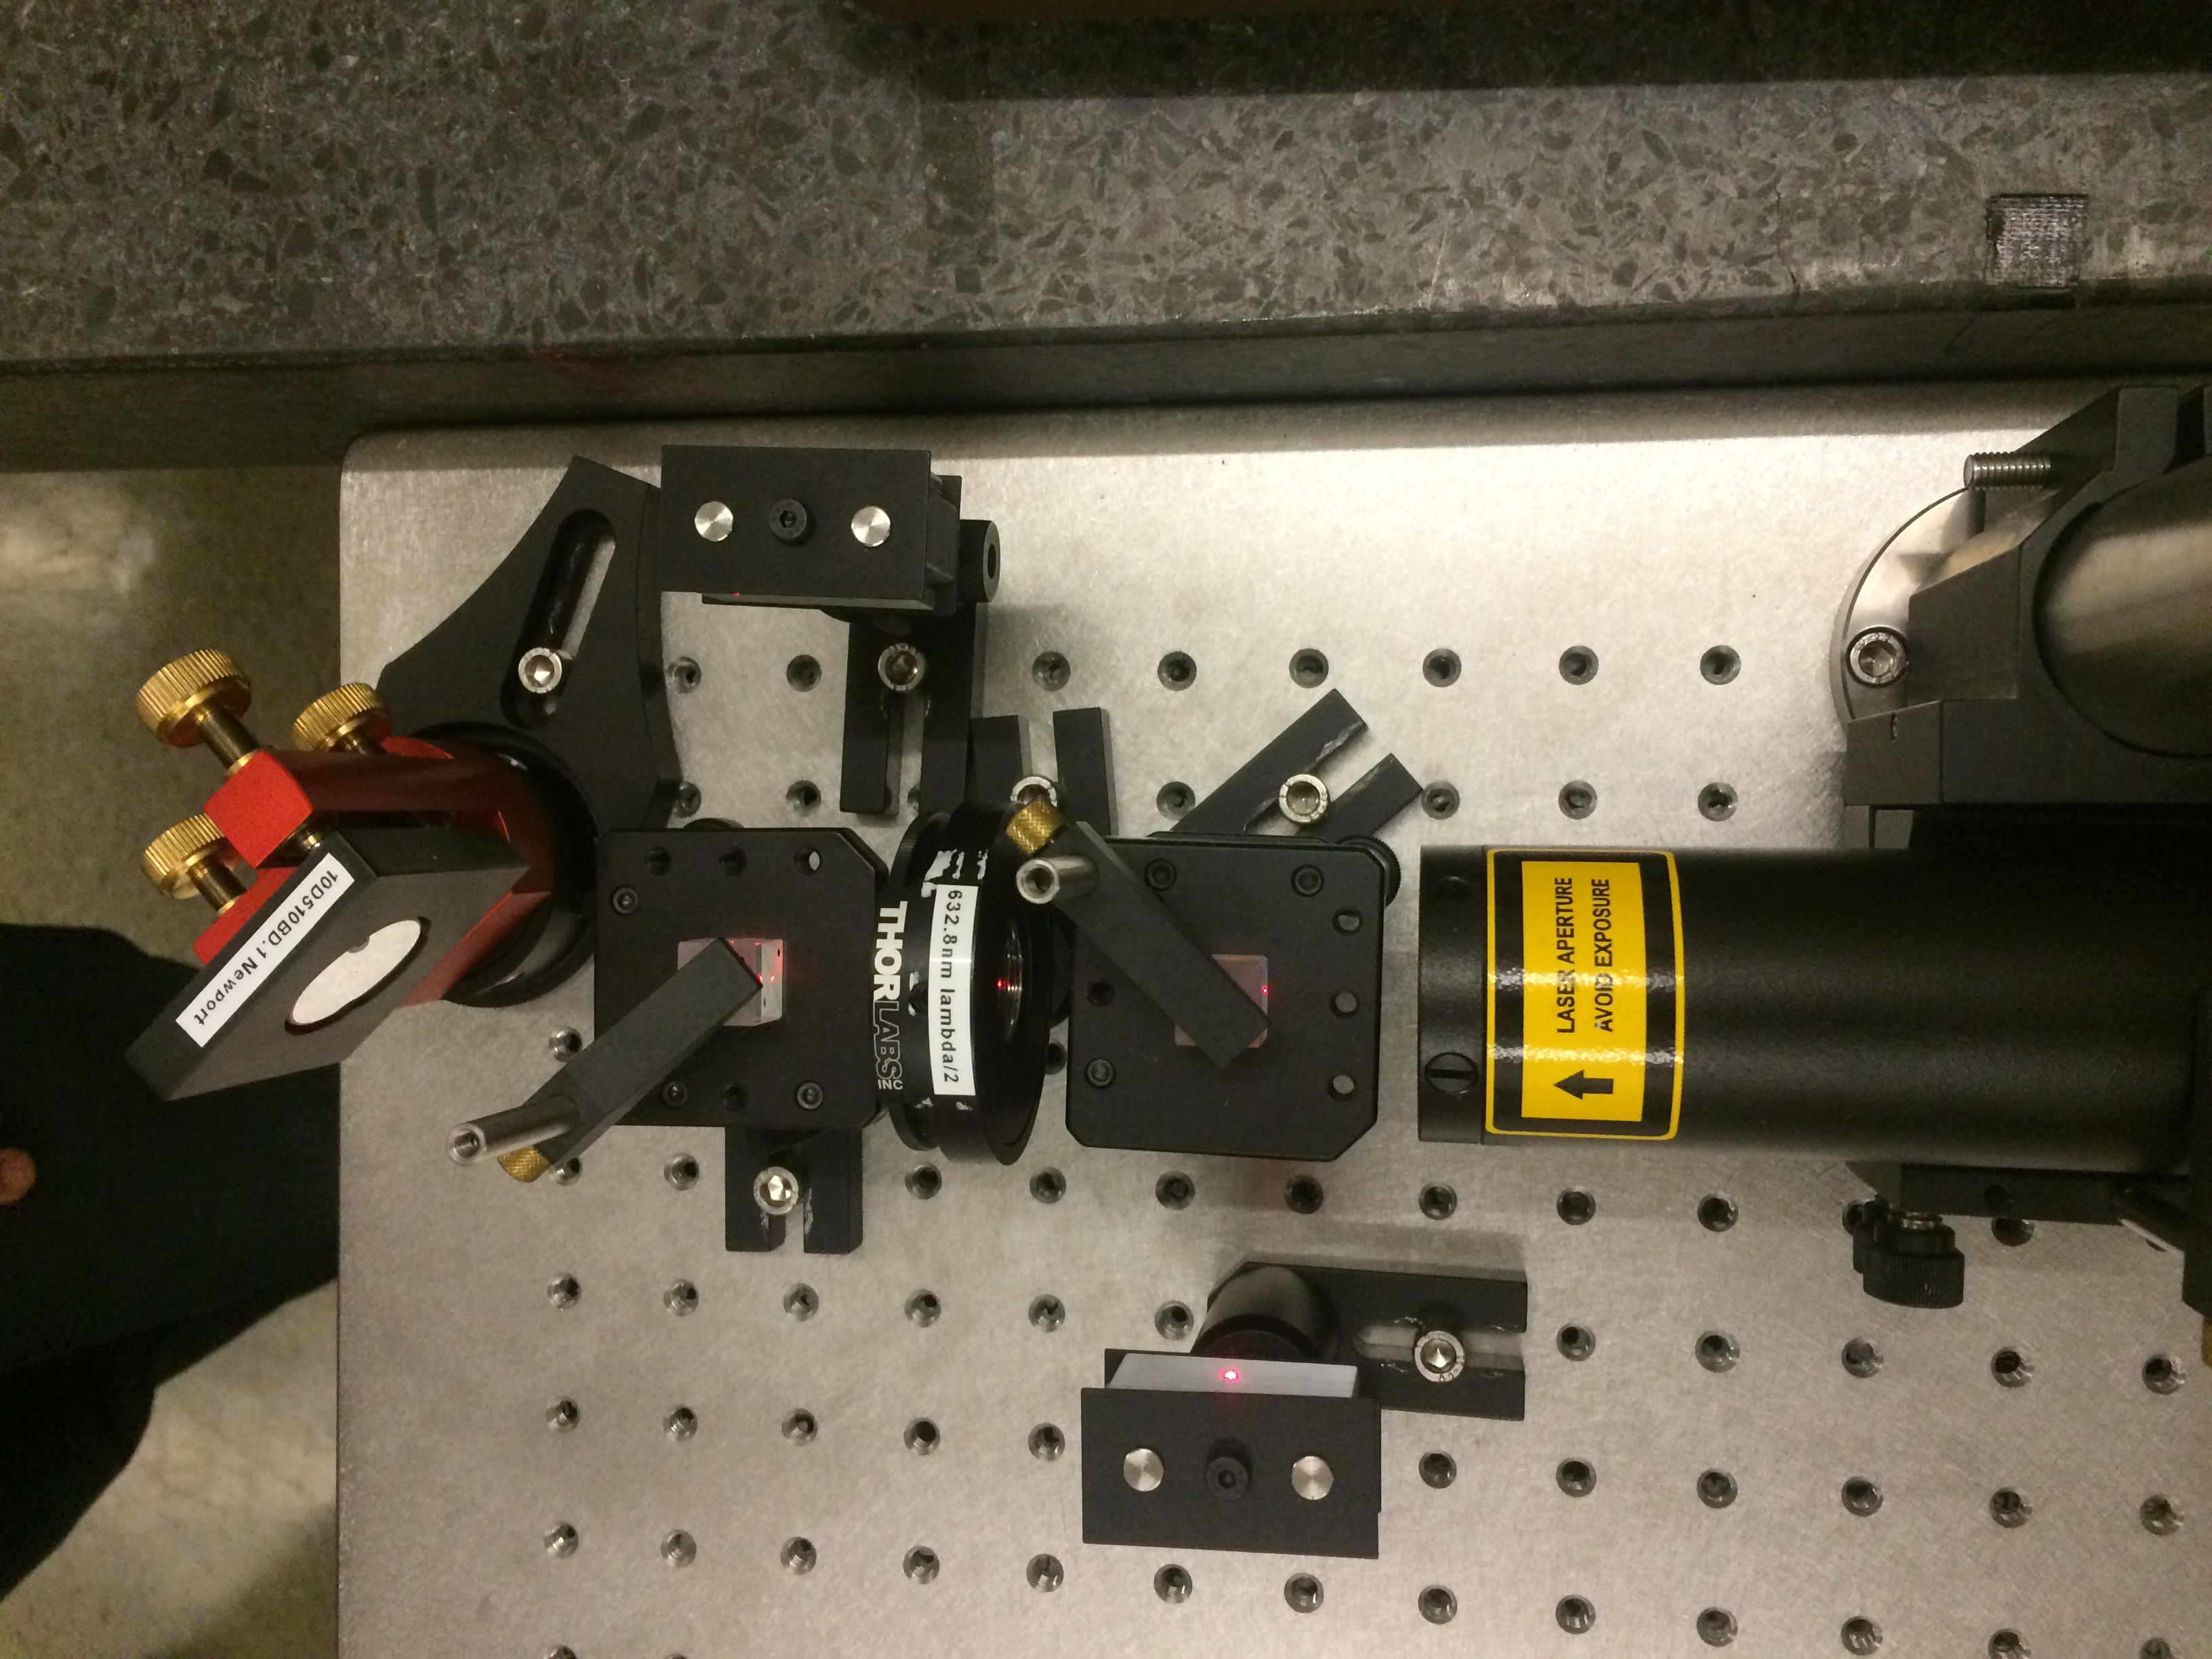
\includegraphics[width=\textwidth, angle=180]{oppsett_photo}
\end{center}
\end{frame}

\begin{frame}[fragile]
\begin{center}
\vspace{0.2cm}
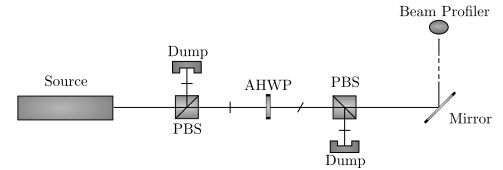
\includegraphics[width=\textwidth]{oppsett1}
\end{center}
\end{frame}

\begin{frame}[fragile]
{\large \color{DarkFern} Ser at profilen er tiln�rmet gaussisk }
\begin{center}
\vspace{0.2cm}
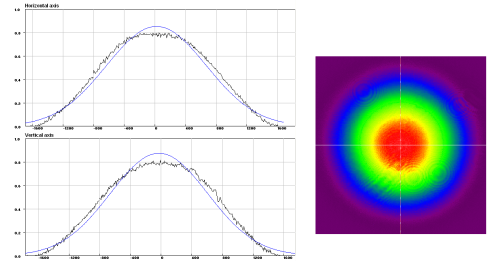
\includegraphics[width=\textwidth]{beampro}
\end{center}
\end{frame}


\begin{frame}[fragile]
{\large \color{DarkFern} Bruker TMA for � tiln�rme krumningsradien }
\begin{center}
\vspace{0.2cm}
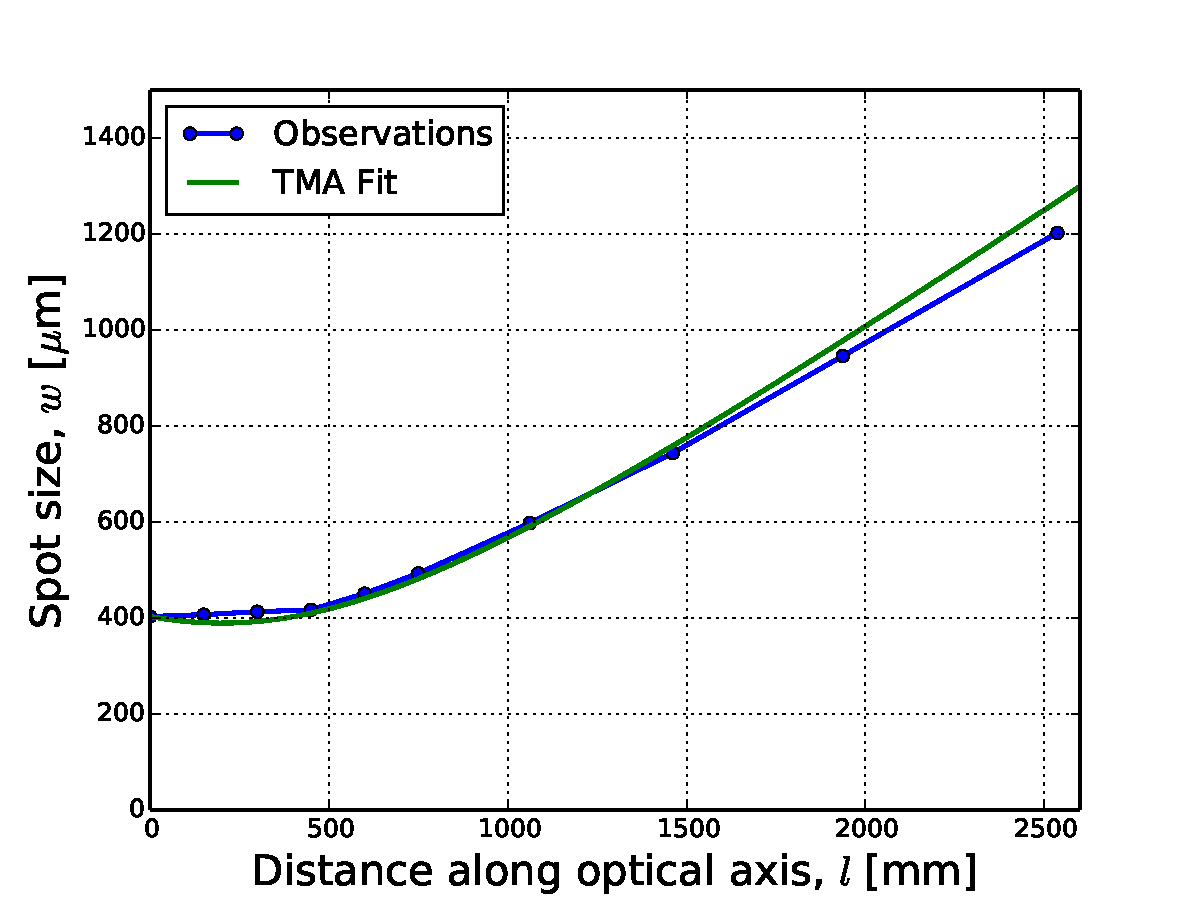
\includegraphics[width=\textwidth]{experiment_1}
\end{center}
\end{frame}

\begin{frame}[fragile]
{\large \color{DarkFern} Tester str�len i n�rheten av midjen}
\begin{center}
\vspace{0.2cm}
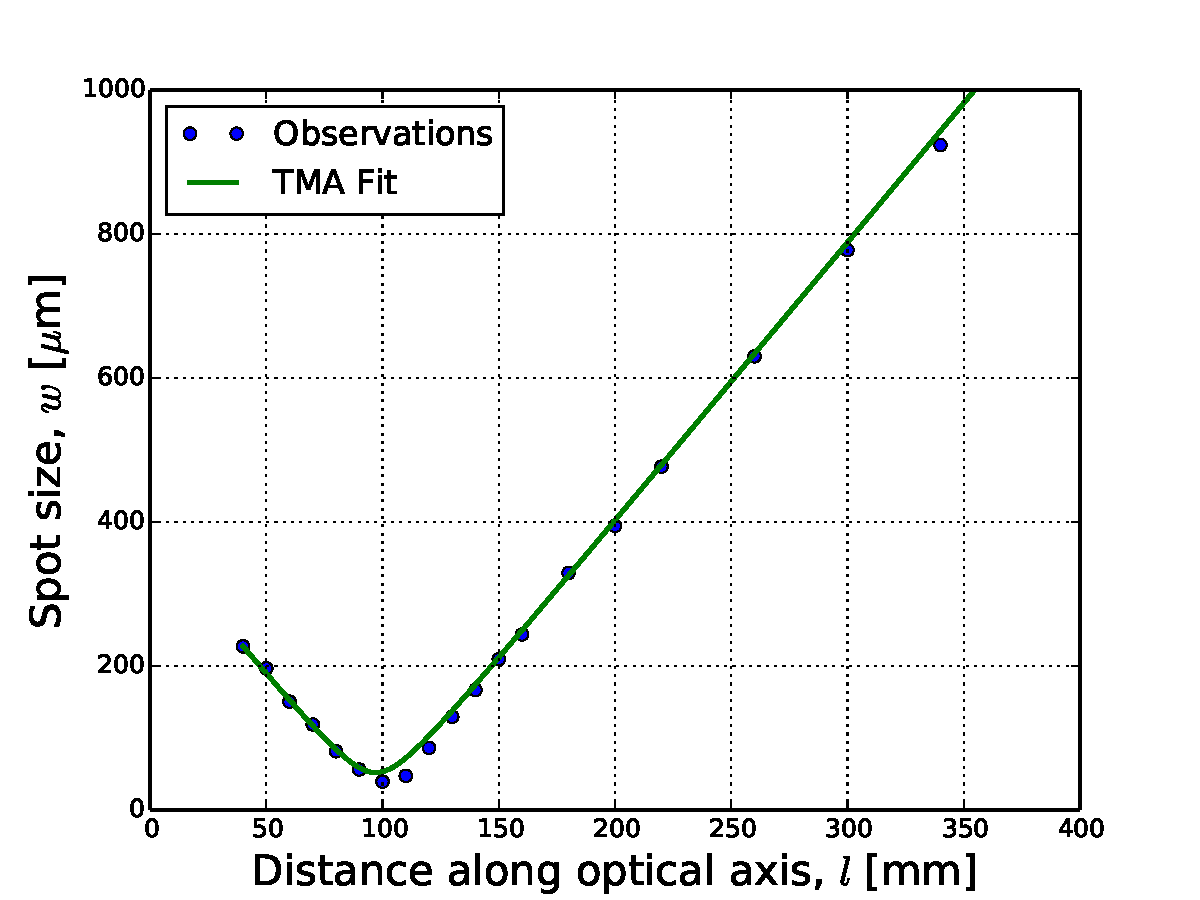
\includegraphics[width=\textwidth]{experiment_1_wlens}
\end{center}
\end{frame}

\begin{frame}[fragile]
{\large \color{DarkFern} Lager en beam expander der avstanden sm�justeres}
\begin{center}
\vspace{0.2cm}
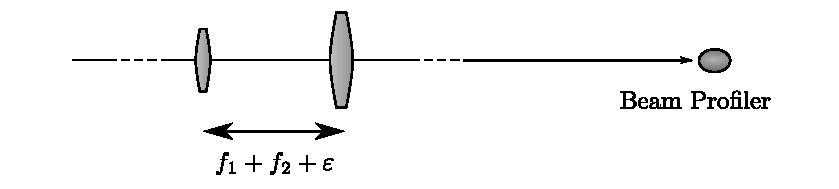
\includegraphics[width=\textwidth]{oppsett2}
\end{center}
\end{frame}


\begin{frame}[fragile]
{\large \color{DarkFern} Avstanden har mye � si for den endelige krumningen}
\begin{center}
\vspace{0.2cm}
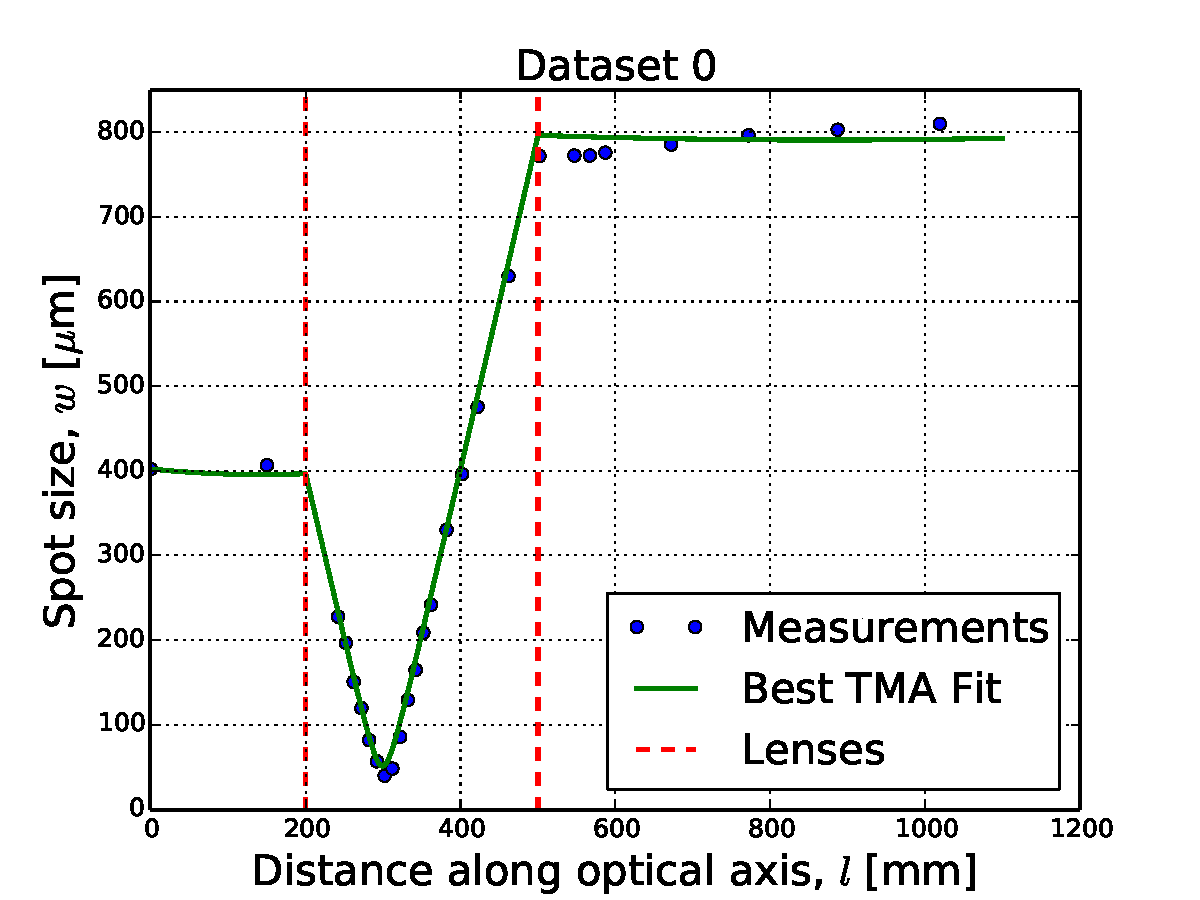
\includegraphics[width=\textwidth]{beam_expander_dataset_0.pdf}
\end{center}
\end{frame}

\begin{frame}[fragile]
{\large \color{DarkFern} Avstanden har mye � si for den endelige krumningen}
\begin{center}
\vspace{0.2cm}
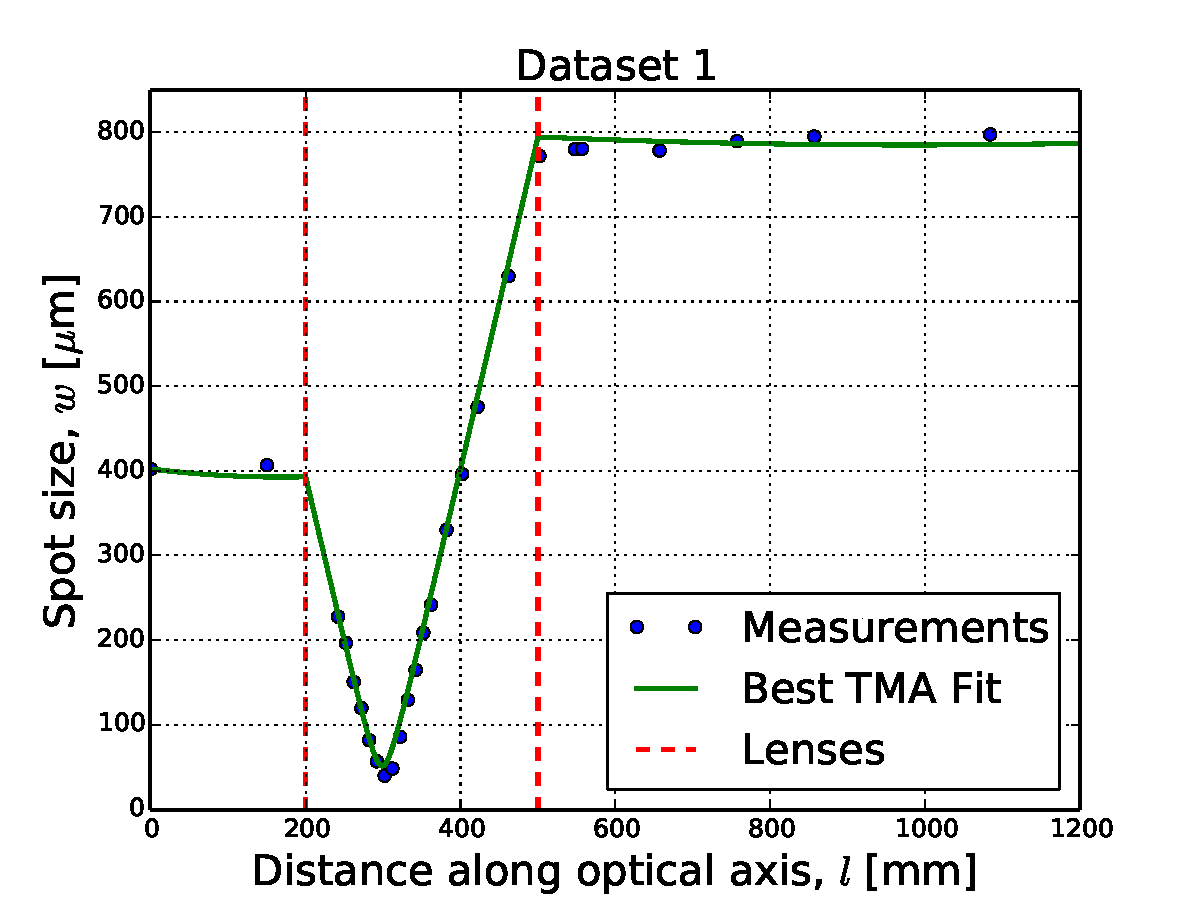
\includegraphics[width=\textwidth]{beam_expander_dataset_1.pdf}
\end{center}
\end{frame}

\begin{frame}[fragile]
{\large \color{DarkFern} Avstanden har mye � si for den endelige krumningen}
\begin{center}
\vspace{0.2cm}
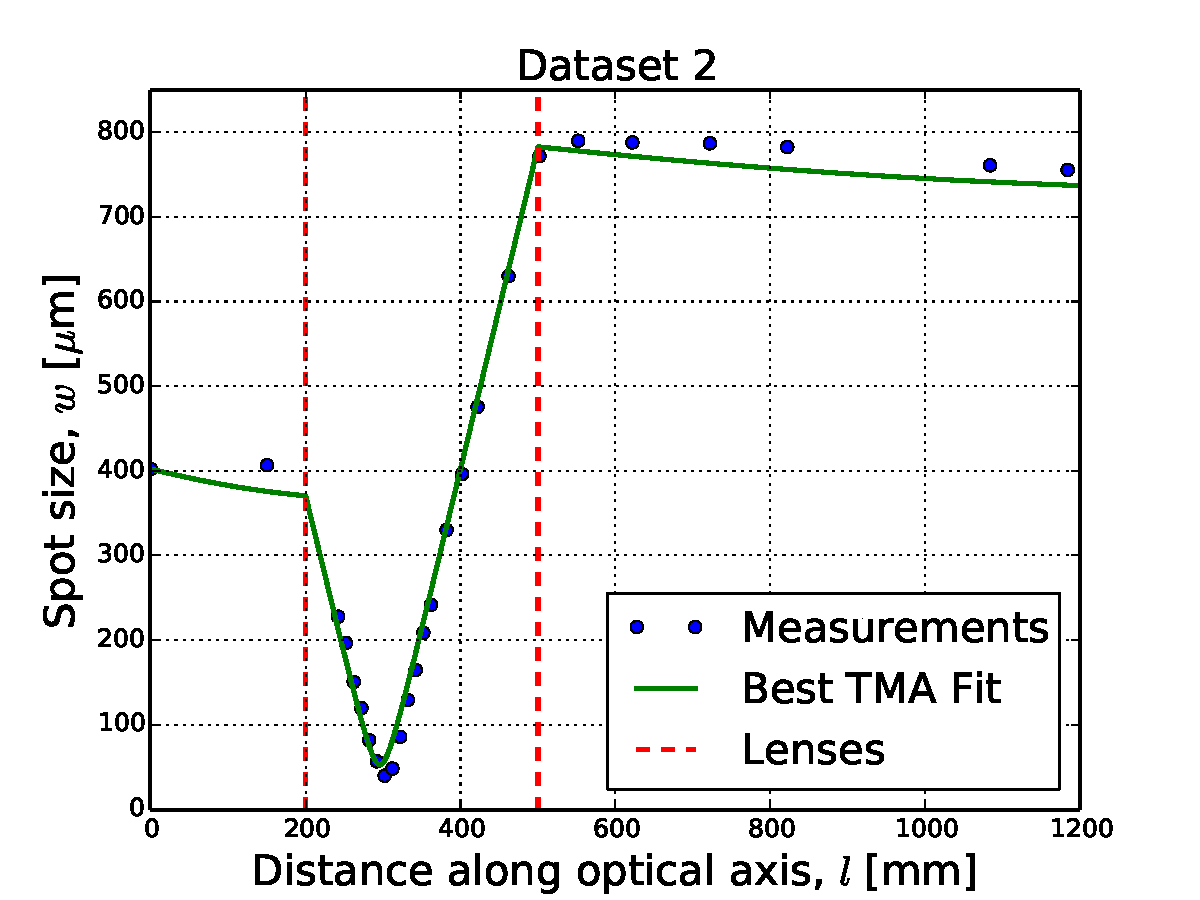
\includegraphics[width=\textwidth]{beam_expander_dataset_2.pdf}
\end{center}
\end{frame}

\begin{frame}[fragile]
{\large \color{DarkFern} Skal sende str�len fra en laserpenn en lang avstand}
\begin{center}
\vspace{0.2cm}
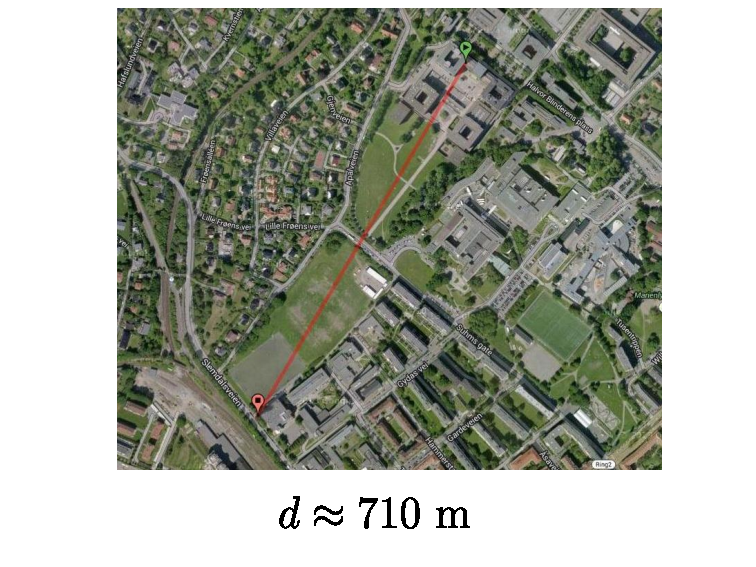
\includegraphics[width=\textwidth]{maps.pdf}
\end{center}
\end{frame}

\begin{frame}[fragile]
{\large \color{DarkFern} Et teleskop brukes som beam expander}
\begin{center}
\vspace{0.2cm}
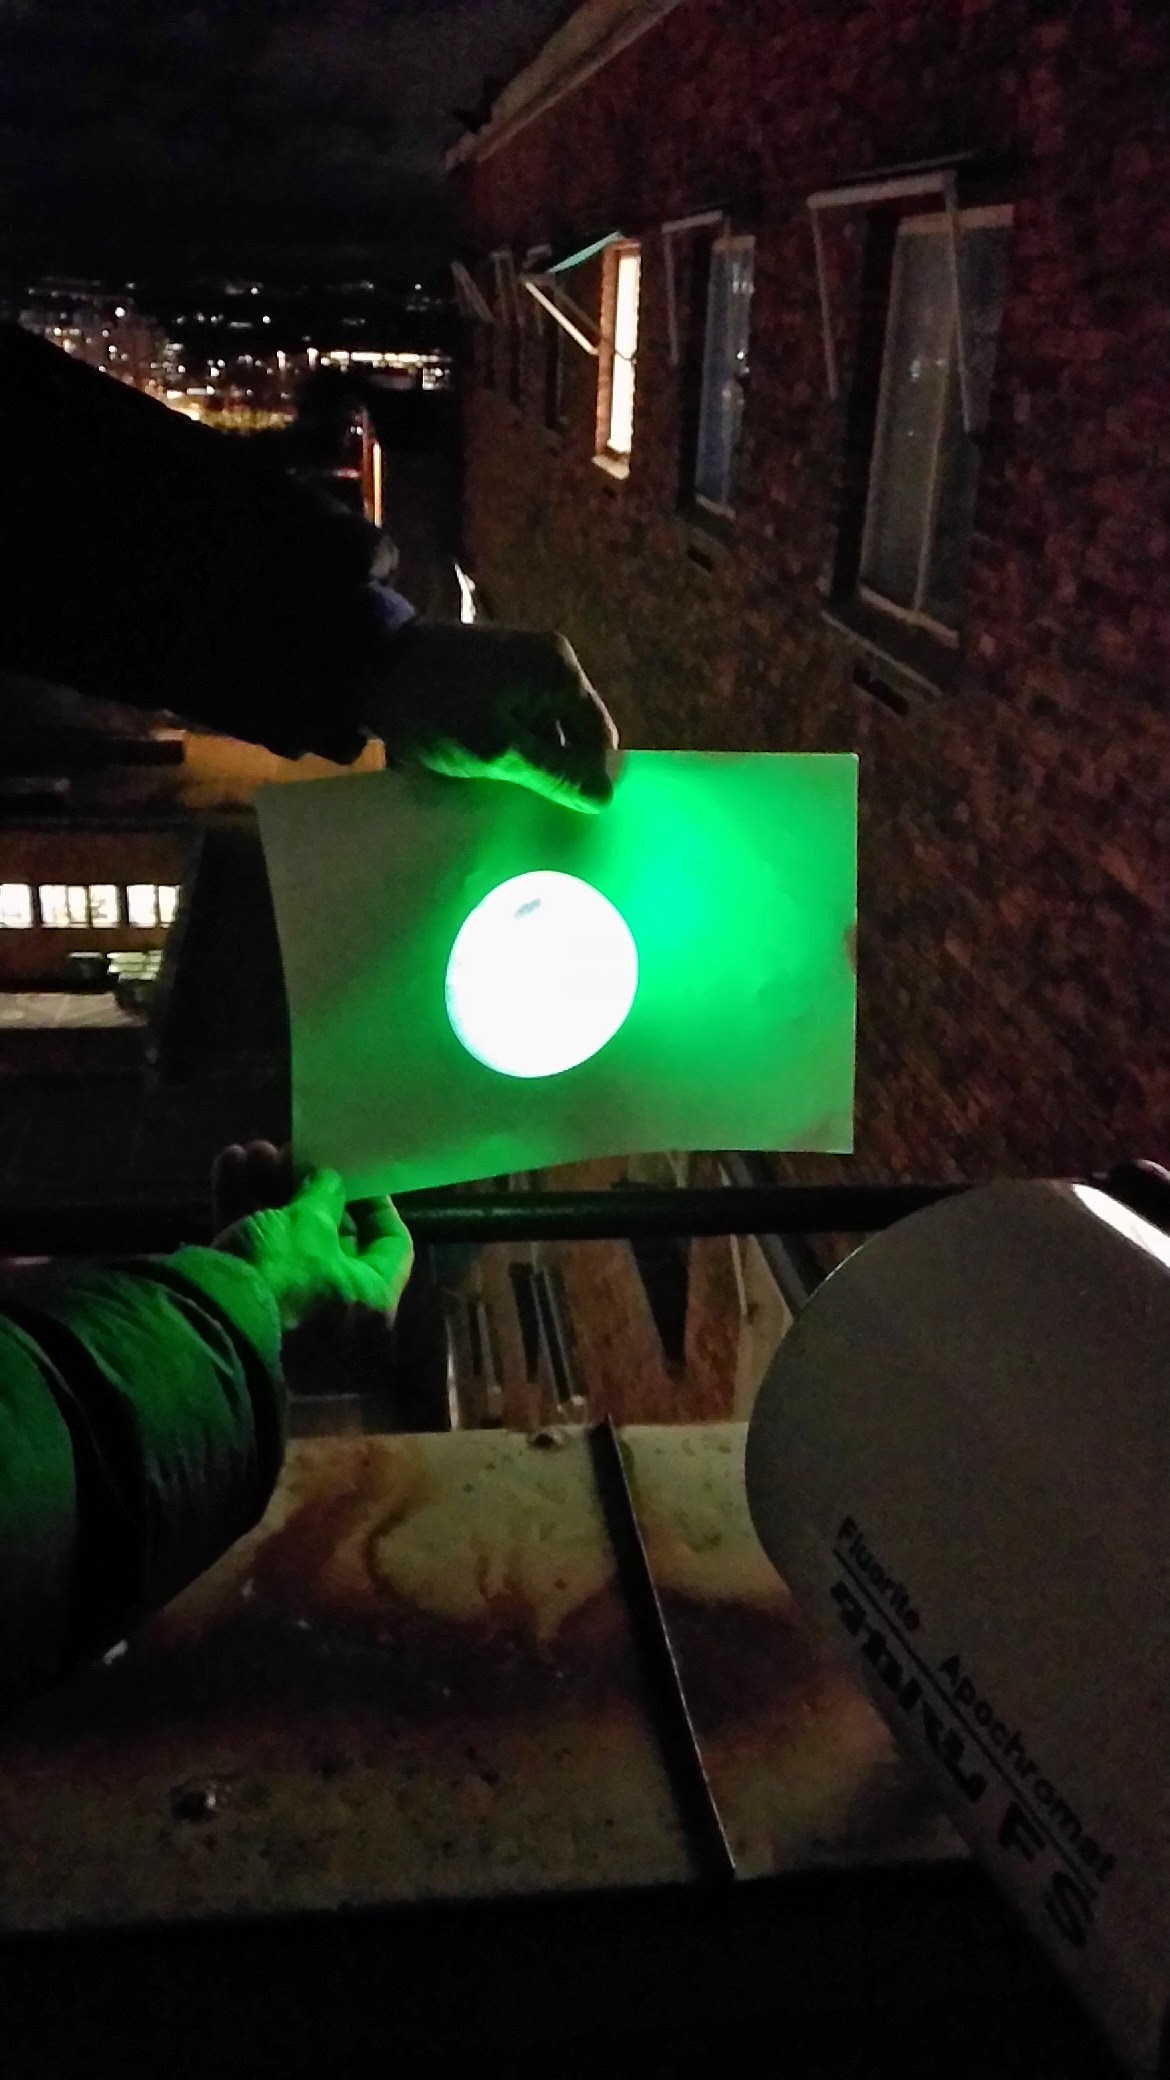
\includegraphics[width=0.4\textwidth]{teleskop}
\end{center}
\end{frame}

\begin{frame}[fragile]
{\large \color{DarkFern} Str�len som starter bredt har lav divergensvinkel}
\begin{center}
\vspace{0.2cm}
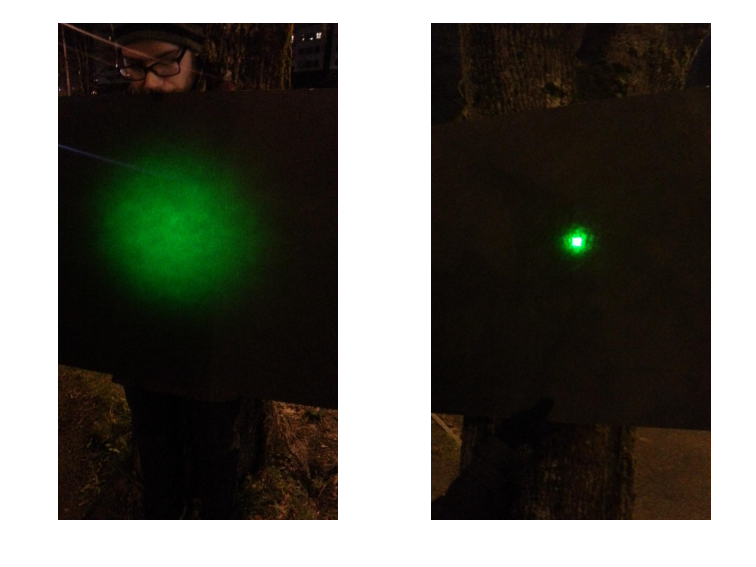
\includegraphics[width=\textwidth]{experiment3.pdf}
\end{center}
\end{frame}

\begin{frame}[fragile]

\vspace{1cm}

{\color{DarkCharcoal} Gaussiske str�ler har gunstige egenskaper som gj�r dem meget lette � regne p�, og gj�r dem gunstige i industri.}

\vspace{1cm}

{\color{DarkCharcoal} Str�legangen kan forutsies av TMA-metoden, men man m� gj�re mange tiln�rminger.}

\vspace{1cm}

{\color{DarkCharcoal} En str�le som skal holde konstant bredde m� starte bredt, dette er fordi $\theta \propto 1/w_0$.}

\vspace{1cm}




\end{frame}



\end{document}